\documentclass[11pt]{article}

% "final" shows the authors' names (no anonymous review version)
\usepackage[final]{acl}

\usepackage{times}
\usepackage{latexsym}
\usepackage[T1]{fontenc}
\usepackage[utf8]{inputenc}
\usepackage{microtype}
\usepackage{inconsolata}
\usepackage{graphicx}
\usepackage{booktabs}
\usepackage{xcolor}


% Red placeholder for anything still to fill in (remove before submission)
\newcommand{\tbd}[1]{\textcolor{red}{[#1]}}

\title{Developing and Comparing Machine Learning Models for Detecting Lean Type 2 Diabetes in Uganda: Locally Trained versus Foreign-Trained Models}

\author{Adriko Patricia Lawuri \\
  2026/HD05/22740U \\
  2600722740 \\
  Makerere University, Kampala \\\And
  Kasadha Jesse \\
  2026/HD05/22756U \\
  2600722756 \\
  Makerere University, Kampala \\}

\begin{document}
\maketitle

% ---------------------------------------------------------------
\begin{abstract}
About a third of Ugandans newly diagnosed with type 2 diabetes are lean, yet the majority of diabetes prediction models are trained on foreign data in which obesity is the dominant risk factor. We aimed to develop and compare machine learning models for detecting diabetes in Ugandan adults, test whether models trained on Ugandan data perform better than foreign-trained models, particularly in lean adults (BMI $<$ 25 kg/m\textsuperscript{2}), and to identify the features that drive their predictions.
 A model trained on 183,579 US adults (80\% of 229,474 BRFSS 2015 respondents) was compared with models trained on 484 eastern Ugandan outpatients whose diabetes was confirmed by oral glucose tolerance test, and with a model pre-trained on US data and fine-tuned on Ugandan data.
 Five algorithms were compared with repeated stratified cross-validation, and all models were tested externally on 3,410 adults from the WHO STEPS Survey, Uganda 2014.
 Only 12\% of people with diabetes in the US data were actually lean, compared with 28\% of the Ugandan outpatients with diabetes and 61\% of people with diabetes in the national survey. Used unchanged in Uganda, the US-trained model detected only 2 of the 23 lean outpatients with diabetes (sensitivity 0.09) and 4 of the 27 lean people with diabetes in the national survey. Logistic regression trained on Ugandan data performed best of the five algorithms (AUC 0.67) and detected 64\% of lean diabetics, rising to 76\% with local features such as waist circumference.
 Foreign diabetes models should not be used in Uganda unchanged. Models trained or at least recalibrated on Ugandan data detect far more lean diabetics.
\end{abstract}

% ---------------------------------------------------------------
\section{Introduction}

Approximately 589 million persons globally had diabetes in 2024; by 2050, that figure is expected to rise to 853 million \citep{genitsaridi2026}. So many patients are diagnosed only after complications such as foot ulcers, blindness, and kidney failure have begun. In rural Uganda, community screening has found many adults with undiagnosed diabetes \citep{10.1093/inthealth/ihaf050}, and laboratory testing is costly and concentrated in urban facilities.
Machine learning models can flag people at high risk for a confirmatory blood test using information collected without a laboratory \citep{xie2019building}. However, most published models are trained on foreign data, typically the Pima Indians dataset \citep{smith1988pima} or US surveys, in which diabetes is closely linked to obesity or being overweight. Diabetes in Uganda differs: in the Uganda Diabetes Phenotype (UDIP) study, about a third of adults with newly diagnosed type 2 diabetes were lean, and their diabetes was linked to low insulin secretion rather than obesity \citep{kibirige2022understanding, kibirige2022apparent}. A model that has learned that ``high BMI means diabetes'' may therefore miss lean patients. A related open-source project has compared US, German, and Ugandan survey data with SHAP \citep{andanter_repo}, but did not focus on lean patients or use a confirmatory glucose test.
This study aimed to develop and compare machine learning models for detecting type 2 diabetes in Ugandan adults, with a focus on lean adults. Specifically, we asked: (1) which of five algorithms (logistic regression, decision tree, random forest, XGBoost and support vector machine) performs best on Ugandan data; (2) do models trained on Ugandan data detect diabetes, especially in lean adults, better than models trained on foreign data; and (3) which features drive the predictions of foreign-trained and locally trained models?


\section{Methods}

\subsection{Data sources}

\paragraph{Foreign data.} The CDC Diabetes Health Indicators dataset contains 253,680 responses to the 2015 US Behavioral Risk Factor Surveillance System (BRFSS) telephone survey \citep{cdc2017dataset}. Diabetes is self-reported, and prediabetes is counted as no diabetes. It is open source

\paragraph{Local training data.} \citet{kasujja2022} studied adults attending the outpatient department of a general hospital in eastern Uganda; every participant had an oral glucose tolerance test (OGTT), the clinical reference test. The data is openly available \citep{kasujja2022data}. Diabetes was defined by WHO criteria: 2-hour OGTT glucose $\geq$ 11.1 mmol/L or fasting plasma glucose $\geq$ 7.0 mmol/L.

\paragraph{Local test data.} The WHO STEPS Survey, Uganda 2014 is a national survey of adults aged 18--69 with measured height, weight, blood pressure and capillary fasting glucose \citep{riley2016steps, moh2014steps}. Diabetes was defined as fasting glucose $\geq$ 7.0 mmol/L or current treatment. The data file was obtained from a public GitHub repository \citep{andanter_repo}; our access request to the WHO NCD Microdata Repository (18 November 2026) is pending.

 The two Ugandan datasets complement each other. The Kasujja data confirm diabetes with the reference test and contain enough cases (82) to train models, but come from a single hospital and include mostly women. The STEPS data represent the national adult population, in which most diabetics are lean, but contain too few cases (44) for training. We therefore trained models on the Kasujja data and used STEPS only as an independent external test, as recommended for prediction models \citep{collins2015tripod}, so that the findings do not depend on a single clinic population.

\subsection{Data preprocessing and exploration}

Duplicate rows were removed from BRFSS (24,206 rows), leaving 229,474 adults. In the Kasujja data, 20 patients had been recorded twice under different study IDs with identical measurements; removing them left 484 patients. In STEPS, glucose codes 77 and 777 (``don't know'') were set to missing, and adults without a glucose result or with an implausible BMI were excluded, leaving 3,410 adults.

Five features are available in all three datasets: age, sex, BMI, high blood pressure, and physical activity. BMI and blood pressure were measured in both Ugandan datasets (high blood pressure: mean of the second and third readings $\geq$ 140/90 mmHg, or treatment in STEPS) but self-reported in BRFSS. The Kasujja data also contain waist circumference, blood pressure readings, and family history of diabetes, used as additional local features. Glucose, HbA1c, and OGTT values were never used as features, because they define the outcome. Exploration compared the three populations, with a focus on the BMI of people with diabetes.

\subsection{Model development}

All models predict diabetes and were evaluated on Ugandan adults:
\begin{itemize}\itemsep0pt
\item \textbf{A. Foreign:} XGBoost \citep{chen2016xgboost} trained on BRFSS with the five shared features. Its threshold was chosen on a 20\% US hold-out set (Experiment A), or alternatively on Ugandan data (Experiment A$'$),to test whether the model's poor performance in Uganda came from the model itself or only from its threshold.
\item \textbf{B. Local:} logistic regression (interpretable baseline), decision tree, random forest, XGBoost and RBF-kernel SVM trained on the Kasujja data, with class weights to counter the 17\% diabetes rate. The best algorithm was then refitted with all local features.
\item \textbf{C. Pre-train and fine-tune:} the US XGBoost model (300 trees) was trained further with 100 additional trees on Ugandan data only.
\item \textbf{D. External test:} the final models were tested on STEPS, which none had seen.
\end{itemize}

\subsection{Model evaluation}

The Ugandan sample is small \citep{kasujja2022data}, models were evaluated with stratified 5-fold cross-validation repeated 10 times. In each training fold, the screening threshold was set by inner 3-fold cross-validation as the highest threshold that detected at least 80\% of diabetics, since a missed diabetic is more harmful than an unnecessary blood test. We report the area under the ROC curve (AUC), sensitivity, specificity, precision and F1 score, as the mean across repeats with the 95\% range, for all patients, lean and non-lean patients, and women and men. SHAP values \citep{lundberg2017shap} were used to compare what the US and Ugandan models rely on.

\section{Results}

\subsection{How common is lean diabetes?}

Lean adults made up 11.6\% of diabetics in the US data, 28.0\% in the Ugandan outpatients and 61.4\% in the national survey (Table~\ref{tab:populations}, Figure~\ref{fig:bmi}). Most US diabetics (58.3\%) were obese. Among the outpatients, the diabetes rate rose from 9.9\% in lean patients to 25.9\% in obese patients; compared with those without diabetes, patients with diabetes were older (51.8 vs 47.2 years) and had higher systolic blood pressure (139 vs 129 mmHg) and a larger waist (95 vs 88 cm)

\begin{table}[t]
\centering\small
\begin{tabular}{@{}lrrr@{}}
\toprule
 & US & Kasujja & STEPS \\
\midrule
People & 229,474 & 484 & 3,410 \\
Diabetics & 35,097 & 82 & 44 \\
Diabetes rate (\%) & 15.3 & 16.9 & 1.3 \\
Men (\%) & 43.9 & 21.5 & 41.9 \\
Mean BMI & 28.7 & 26.1 & 22.9 \\
Lean, all adults (\%) & 27.0 & 48.1 & 78.0 \\
\textbf{Lean, diabetics (\%)} & \textbf{11.6} & \textbf{28.0} & \textbf{61.4} \\
\bottomrule
\end{tabular}
\caption{The three study populations after cleaning. Lean = BMI $<$ 25 kg/m\textsuperscript{2}.}
\label{tab:populations}
\end{table}

\begin{figure}[t]
\centering
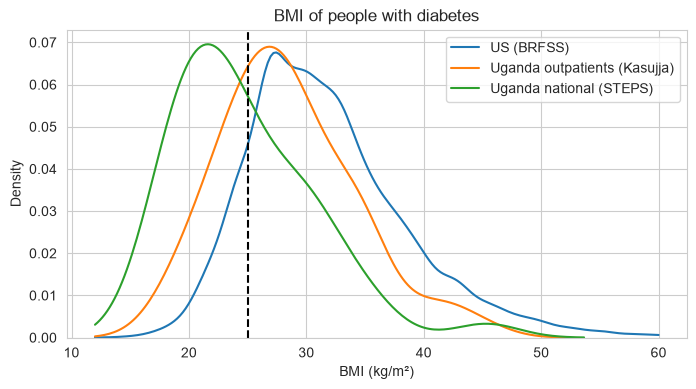
\includegraphics[width=\columnwidth]{figures/bmi_of_diabetics.png}
\caption{BMI of people with diabetes in each dataset. The dashed line marks the lean cut-off (25 kg/m\textsuperscript{2}).}
\label{fig:bmi}
\end{figure}

\subsection{Predictive models for diabetes}

Of the five algorithms trained on Ugandan data, logistic regression had the highest AUC (0.668), followed by random forest (0.661), XGBoost and SVM (0.641) and the decision tree (0.637) (Table~\ref{tab:algorithms}). All detected 81--87\% of diabetics overall, but only 49--65\% of lean diabetics.

\begin{table}[t]
\centering\small
\begin{tabular}{@{}lccccc@{}}
\toprule
Model & AUC & Sens. & Spec. & F1 & Lean sens. \\
\midrule
Logistic regression & \textbf{0.668} & 0.843 & 0.366 & 0.341 & 0.635 \\
Random forest & 0.661 & 0.812 & 0.427 & 0.351 & 0.487 \\
XGBoost & 0.641 & 0.865 & 0.350 & 0.342 & 0.648 \\
SVM (RBF) & 0.641 & 0.837 & 0.341 & 0.330 & 0.617 \\
Decision tree & 0.637 & 0.839 & 0.355 & 0.335 & 0.609 \\
\bottomrule
\end{tabular}
\caption{Performance of five algorithms trained on Ugandan outpatients (shared features; mean of 10 repeats of 5-fold cross-validation).}
\label{tab:algorithms}
\end{table}

Applied unchanged with its US threshold, the  model (hold-out AUC in the US 0.771) detected only 37.8\% of Ugandan diabetics and 2 of 23 lean diabetics (sensitivity 0.087), compared with 49.2\% of non-lean diabetics (Table~\ref{tab:main}, Figure~\ref{fig:lean}). Its AUC on Ugandans (0.689) was similar to that of the local models, so its main failure was its threshold. With a threshold chosen on Ugandan data, it detected 80\% of all diabetics but still only 56.5\% of lean diabetics. The local logistic regression detected 63.5\% of lean diabetics with the same five features and 75.7\% with all local features. Pre-training and fine-tuning did not improve on the local model (AUC 0.652; lean sensitivity 0.622). Precision was low for every approach (20--34\%).

\begin{table}[t]
\centering\small
\begin{tabular}{@{}lcccc@{}}
\toprule
 & \multicolumn{2}{c}{All (82)} & \multicolumn{2}{c}{Lean (23)} \\
Approach & AUC & Sens. & AUC & Sens. \\
\midrule
A. Foreign, US thr. & 0.689 & 0.378 & 0.646 & \textbf{0.087} \\
A$'$. Foreign, Ugandan thr. & 0.689 & 0.796 & 0.646 & 0.565 \\
B. Local LR, shared & 0.668 & 0.843 & 0.611 & 0.635 \\
B. Local LR, all local & 0.682 & 0.915 & 0.602 & \textbf{0.757} \\
C. Fine-tuned & 0.652 & 0.849 & 0.571 & 0.622 \\
\bottomrule
\end{tabular}
\caption{Foreign, local and fine-tuned models on the Ugandan outpatients (number of diabetics in brackets). LR = logistic regression; thr. = threshold.}
\label{tab:main}
\end{table}

\begin{figure*}[t]
\centering
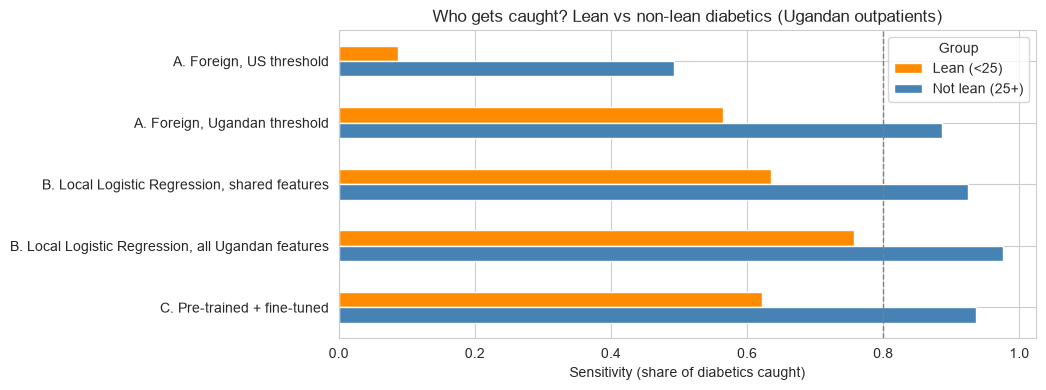
\includegraphics[width=0.85\textwidth]{figures/lean_sensitivity.png}
\caption{Share of lean and non-lean diabetics detected by each approach (Ugandan outpatients). The dashed line marks the 80\% target.}
\label{fig:lean}
\end{figure*}

\subsection{External test on the national survey}

On the STEPS national sample, all models had similar AUC (0.70--0.71). With its US threshold, the US model detected 4 of 27 lean diabetics (14.8\%) but 11 of 17 non-lean diabetics (64.7\%). The local model and the US model with a Ugandan threshold each detected 11 of 27 lean diabetics (40.7\%), and the fine-tuned model detected 16 of 27 (59.3\%). Because only 1.3\% of this sample had diabetes, precision was 2--5\%.

\subsection{Interpretation of results}

The US model relied most on high blood pressure (35\% of total SHAP importance) and BMI (30\%), whereas a Ugandan XGBoost model relied most on age (38\%) and BMI (35\%). For lean Ugandan diabetics, BMI lowered the predicted risk on average by 0.86 in the US model but by 0.31 in the Ugandan model, and age lowered the risk in the US model ($-$0.28) but raised it in the Ugandan model (+0.23). In the US model, risk falls steadily with every unit of BMI below 30 (Figure~\ref{fig:shap}), which is why lean diabetics fall below its threshold.

\begin{figure*}[t]
\centering
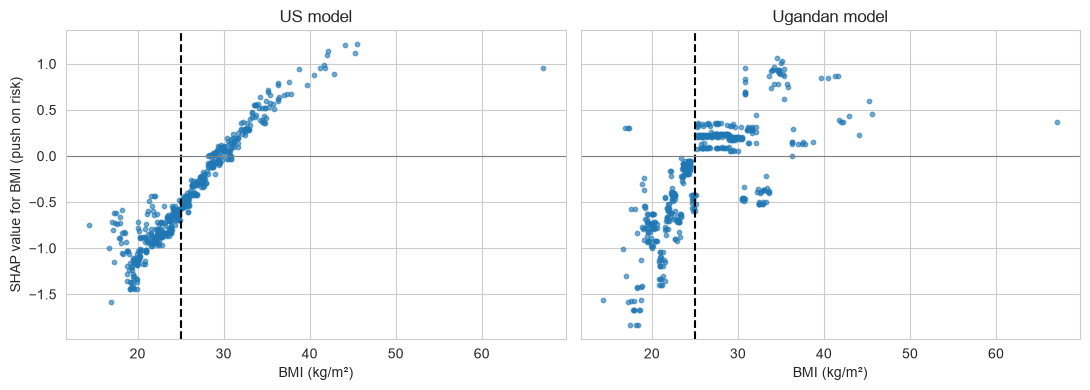
\includegraphics[width=0.85\textwidth]{figures/shap_bmi_dependence.png}
\caption{SHAP dependence of BMI in the US and Ugandan models, explained on the Ugandan outpatients. Negative values push the predicted risk down. The dashed line marks BMI 25.}
\label{fig:shap}
\end{figure*}

% ---------------------------------------------------------------
\section{Discussion}

The results support the concern that foreign diabetes models fail lean Ugandans. SHAP shows the mechanism: the US model has learned that a normal BMI means low risk. Two findings refine this conclusion. First, the US model still ranked Ugandan patients about as well as the local models, so much of its failure lies in a threshold set for an obese population.Recalibrating it on Ugandan data recovered many cases. Second, models trained on Ugandan data detected more lean diabetics than the recalibrated US model, and local features such as waist circumference and family history helped further.
The simplest model performed as well as more complex ones: logistic regression outperformed random forest, XGBoost, SVM and the decision tree. Fine-tuning a US model on Ugandan data gave mixed results, with no gain in the outpatients but the highest lean sensitivity in the national survey with 484 training patients, the US starting point may pull the model towards the US pattern.

\paragraph{Limitations.} The training sample is small (82 diabetics, 23 lean) and comes from one hospital whereas the external test has only 44 diabetics, so estimates are uncertain. 
Only 21.5\% of the outpatients were men. Diabetes is self-reported in BRFSS but measured in Uganda, and blood pressure is defined differently, so part of the foreign local difference may reflect these definitions.
Neither Ugandan dataset records diabetes type. Only five features were shared, which limits AUC; precision was low, so the tool can only decide who needs a confirmatory blood test.

\section{Conclusion}

Of five algorithms trained on Ugandan data, interpretable logistic regression performed best, ahead of random forest, XGBoost, SVM and the decision tree. A diabetes model trained on US data and applied unchanged to Ugandans missed about 9 in 10 lean diabetics, whereas models trained on Ugandan data detected up to three quarters of them. SHAP showed why the US model relies on BMI and treats a normal BMI as low risk, while the Ugandan model gives more weight to age. Diabetes screening tools for Uganda should be trained, or at least recalibrated, on Ugandan data and should not depend on BMI. Larger Ugandan datasets with confirmed diabetes, such as those of the UDIP and DOP studies, are needed to confirm these findings.

\paragraph{Future work:} 
Embedding the model in electronic medical records. Uganda's public health facilities already use electronic medical record (EMR) systems, on average 4.8 per facility across 265 government facilities \citep{ddamba2025}. The final model uses measurements routinely taken at triage (age, sex, height, weight, waist circumference, blood pressure, family history and physical activity), and logistic regression reduces to a single weighted formula, it could be built into an EMR such as UgandaEMR as a decision-support rule that runs without internet access and shows which factors raised a patient's score. 

In practice, the score would be calculated as vital signs are entered; patients above the threshold, including lean patients, would be flagged for a confirmatory fasting glucose or HbA1c test; and the confirmed results recorded in the EMR would provide new Ugandan data for retraining the model. Before deployment, the model needs validation on larger Ugandan data, prospective testing in clinics, an assessment of the extra testing workload, ethical and Ministry of Health approval, and attention to the limited interoperability between existing EMR systems, which was reported in only 10\% of facilities \citep{ddamba2025}.

\paragraph{Code availability.} The notebook and code are available at \url{https://github.com/adrikopatty/lean-diabetes-Uganda}. The Kasujja data are openly available on Figshare; the STEPS data can be requested from the WHO NCD Microdata Repository.

\bibliography{custom}

\end{document}
